\documentclass[12pt]{article}
\usepackage{fixltx2e}
\usepackage{float}
\newcommand{\degree}{\ensuremath{^\circ}}
\usepackage{graphicx}
\usepackage[margin=1.0in]{geometry}
\usepackage{amsmath}


\title{Portfolio Optimization in Python}
\author{Michael Lee \\*
BS Mechanical Engineering | BA Economics \\*
The University of Texas at Austin}
\date{Fall 2013}

\begin{document}
\maketitle{}
Portfolio management can be viewed as an optimization problem in which profit is maximized subject to a limit on volatility. In the proposed model, a monte carlo simulation is run to randomly generate portfolio allocations for each asset. The price of each asset is pulled from online sources and this data is used in calculating both profit and volatility. Volatility is calculated using an exponentially weighted moving average, which more strongly weights recent data. The locally optimal solution is the portfolio that has the highest profit without exceeding a predetermined level of risk. The model is run in the Python programming language and takes advantage of \emph{NumPy's} mathematical functions, \emph{Pandas} ability to handle time-series, as well as the \emph{Statsmodels'} statistical capabilities.

\newpage
\section{The Base Model}
The original model as developed by Ruben Mercado, Scott Schwaitzberg, and David Kendrick utilizes a monte carlo method to randomly generate the stock prices. The performance of these stocks is simulated by the a random number generator times some coefficient. While this is psuedorandom, ultimately the asset's final price is determined by the hard-coded inital values. This is less than optimal, and misses the complexity that real data has to offer. Also, the covariance of the portfolio is not calculated, thus missing out on an important metric of portfolio diversification. 


\section{Improved Model in Python}
Building off the works of Mercado, Schwaitzberg, and Kendrick, an improved model is created-- one that utilizes real-world stock prices to more accurately simulate portfolio management. Additionally, a different method of calculating asset volatility is built in such that recent volatility is more heavily weighted. The proposed model still utilizes a monte carlo method for optimization, as a closed form function could not be readily created.

\subsection{Pulling Real-Time Data}
Instead of simply creating fictional stock prices and volatility, the new model turns to the web. By interfacing with Yahoo! Finance's api, we are able to pull historical financial data into the model, including the adjusted close price and ${\beta}$, a measure of an asset's covariance with the market (usually defined as the S\&P 500). ${\beta}$ is often used as a proxy for an asset's systemic risk, or the risk posed to all assets in a market segment and cannot be eliminated via portfolio diversification (\emph{LSE}). \\*\\*
From the historical data (01/01/2010 - Present), some basic statistics are calculated, including the mean (${\mu}$), standard deviation (${\sigma}$), and correlation (${\rho}$). Where ${\emph E}$ is the expected value operator:



\begin{equation}
	\mu = \frac{x_{1} + x_{2} ... + x_{n}} {n}
\end{equation}	

\begin{equation}
	\sigma = \sqrt{E[(X - \mu])^{2}}
\end{equation}	
	
\begin{equation}
	\rho_{x,y} = \frac{E(X - E[X])(Y-E[Y])}{\sigma_{x}\sigma_{y}}
\end{equation}

From the above we can evaluate how risky-- and profitable-- our portfolio is. The mean of the asset price over time is used to predict how profitable an asset will be over time; the standard deviation how volatile the asset is; the covariance how diversified our portfolio is. The covariance is particularly important in building a successful portfolio as it shows how the assets fluctuate in unison. A covariance of unity implies that the two assets move in equal amounts-- when the price of one increases the price of the other increases by the same percentage-- a covariance of negative one implies that when the price of one asset increases, the other asset decreases by the same amount. In this model, and optimal total covariance is naught, meaning that the portfolio will perform well regardless of volatility in one particular asset.

\subsection{Exponentially Weighted Moving Average}
While the standard mean is useful in understanding an asset's long-term value, it has major flaws in evaluating future success. An arithimetic mean equally weights recent and distant performance. This causes serious error in assets whose price has risen or fallen dramatically in recent times as an asset is more likely to follow current trends than distant trends. To account for this, an exponentially weighted moving average (EWMA) is taken for each asset. As described by Minkah (Minkah, 2007), the EWMA is defined as:

\begin{equation}
	\sigma = \sqrt{(1-\lambda) \sum{ \lambda^{i}(r_{i-1} - r_{avg})^2})}
\end{equation}

Where \emph{r} is the return on an asset and $\lambda$ is some decay factor. A financial services company, \emph{RiskMetrics}, as does this model,uses a decay factor of .94 in its forcasting. However, $\lambda$ can be changed to reflect the manager's opinion on how distance performance reflects future gains. 

\subsection{Monte Carlo Simulation}
Monte Carlo simulations are often used in financial modeling in situations where a closed-form analytic solution is not readily avaialbe or exceedingly compuationally intensive. A monte carlo simulation relies on repeated random sampling of input variables to obtain an optimal result. In the case of portfolio managment, by randomly chosing the asset allocation percentages and calculating the profit and volitility repeatedly, the law of averages states that as the number of simulations approaches infinity, an optimal solution will be found. \\*
In the proposed model, sampling was done according to the Dirichlet distribution, which ensures that some number of points, \emph{n}, are randomly sampled such that their sum is equal to some specifed total. Thus, the Dirichlet distribution has the statiscally appealing property of being the conjugate prior to the parameters of the multinomial distribution. 

\begin{equation}
	p({\bf p}) = Dirichlet({\bf p, u}) = \frac{1}{Z({\bf u})} \Pi p_{i}^{u_{i}-1}
\end{equation}

\subsection{Defining Optimality}
After repeated random sampling we will have a \emph{m x n} matrix where \emph{n} is the number of runs and \emph{m} houses the variables of interest, namely profit, EWMA, and the weights of each asset in the portfolio. Where $w^{j}$ is the weight of each $j^{th}$ asset:

\[optimal(\pi, \sigma) = \left | \begin{array}{ccc}
\pi_{1} & ... & \pi_{n} \\
\sigma_{1} & ... & \sigma_{n} \\
w_{1}^{1}  & ... & w_{1}^{n} \\
w_{2}^{1}  & ... & w_{2}^{n} \\
... & ... & ... \\
w_{j}^{1}  & ... & w_{j}^{n} \end{array} \right |\]

The optimal porfolio is the one that has the highest profit as defined by:

\begin{equation}
	\pi = \sum{w^{j} *(P_{i}^{j} - P_{f}^{j})}
\end{equation}

However, a good porfolio will also limit the amount of exposure it has to market volitilty. Thus, any portfolio allocation whose combined volitility--as defined by the EWMA-- is greater than a predefined level of risk is elimated from the maximization. The optimization problem is now defined as:

\begin{equation}
	\begin{split} 
		&= max: \pi \\ 
		&= s.t: \sum{\sigma^{j}} < \sigma^{max}
	\end{split}
\end{equation}

The algorithim is designed such that the asset data is pulled once, and the allocation is run \emph{n} times. After the final matrix has been compiled, a search function is first used to eliminate all columns that do not satsify equation 7, then finally to find the column housing maximum profit. For a more detailed look at the full program, consult the appendix. 

\section{Results}
The monte carlo simulation was run 1000 times, taking a total of 15 minutes to computute and generating an output of 37 kb. All results were normalize to buying one share. Some basic statistics of the finalized results {\bf (Note: portfolios not satisfying equation 7 are not figured into any calculations)}:

\begin{itemize}
	\item Average Profit: \$53.05
	\item Std. Dev Profit: \$28.19 
	\item Median Profit: \$46.68
	\item Max Profit: \$176.73 
	\item Average EWMA Standard Dev: \$177.86
\end{itemize}

A plot of the profit vs the EWMA standard deviation is pictured below. It is interesting to note that the highest returning portfolio is one of the least risky as well. While this data is biased by the omission of the highly volitile results, it is informative never the less. 


\begin{figure}[!h]
\begin{center}
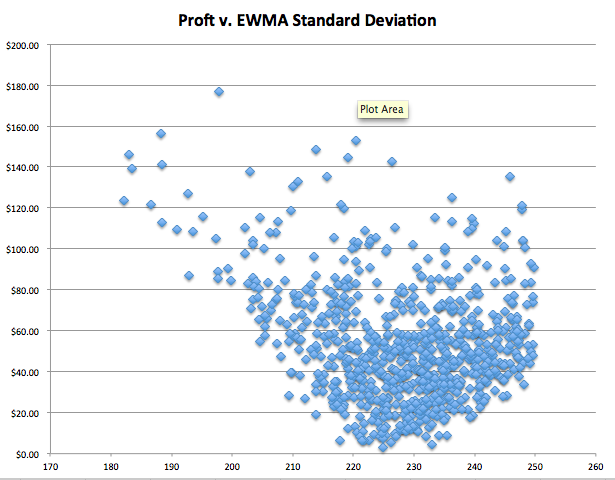
\includegraphics[scale=.5]{Figures/ProfitvVar.png}
\caption{Profit vs. EWMA Standard Deviation}
\end{center}
\end{figure}
\newpage

The respective allocations of the optimal portfolio is pictured below: 

\begin{figure}[!h]
\begin{center}
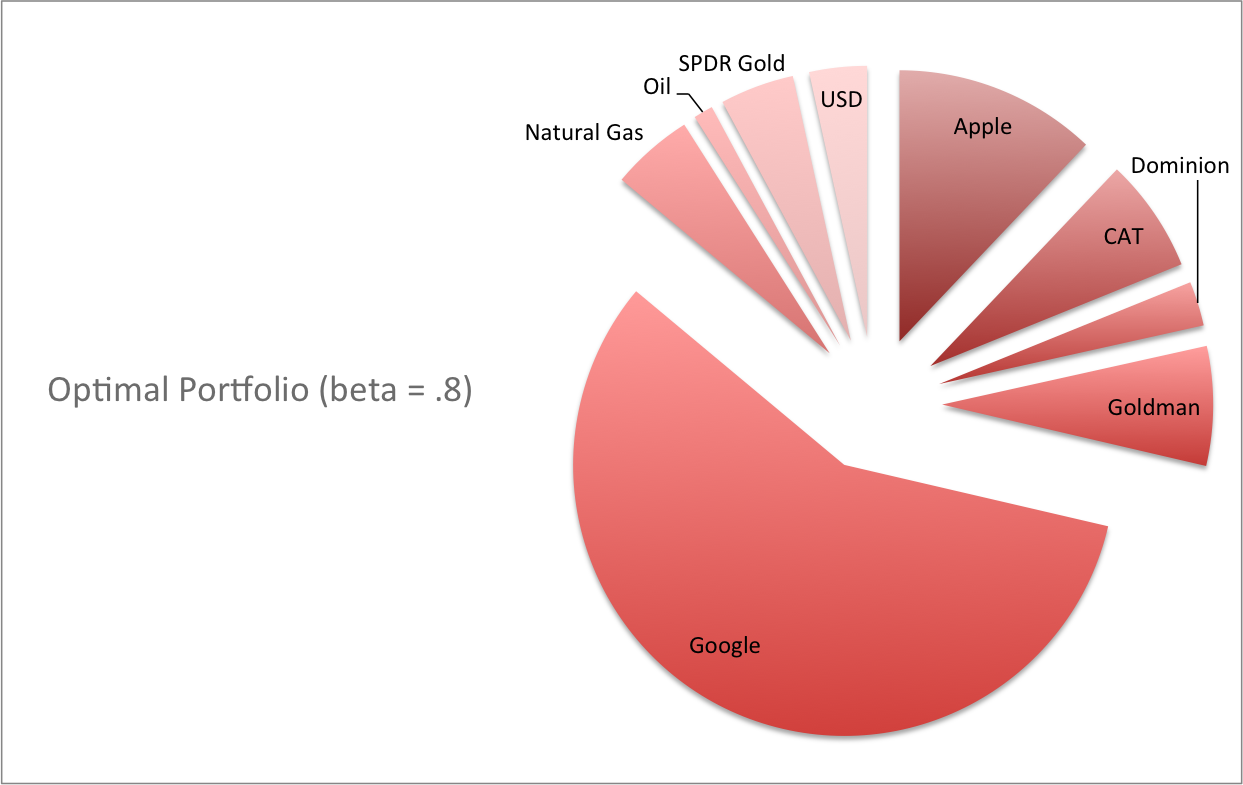
\includegraphics[scale=.5]{Figures/OptimalPort.png}
\caption{The Optimal Portfolio Allocation}
\end{center}
\end{figure}


The impressive rise of Google's share price over time undoubtedly contributed to its majority stake in the simulated portfolio. Goldman Sachs, who at the time of running had a share price of \$160, occupies a relatively small portion of the portfolio because of its high volitlity. In contrast, Catapillar has been incredibly stable recently, so while its share price of \$86 is relatively low, its stability brought down the portfolio's average volitility, allowing it to purchase large quanties of more profitable, but risky shares, such as Apple.

\section{Future Improvements}
Given more time, the model can be improved to become a better forcasting agent by creating a markov chain in which the assest's future performance can be predicted based on deterministic processes. This would allow the model to not only select optimal allocations based on past performance, but become a full-fledged financial tool. \\*
Future iterations of the model can be altered to incorporate non-traditional assets, such as options and derivatives via the Black-Scholes equation. This would allow for a more robust portfolio as these assets have characteristics such as a negative beta, i.e. that they perform well when the market doesn't. \\*
In additon, I would like to explore market betting. By eliminating all the volitile portfolios, many extremely profitable ones are non-factors. I would like to create a seperate metric to constrain the optimization, such as tail-side risk, that will allow for the model to effectively predict and bet on the market's movements in order to increase profit. 

\newpage



\end{document}